\chapter{DISCUSSION}

\section{Behaviour at default parameters}

Across the test set under default parameters, the symmetric Hausdorff error stays under 1\% of the bounding-box diagonal on the sphere and torus tests, and the per-iteration cost of the diffusion solver remains low because of the one-time Cholesky factorisation. The spherical-cap displacement model produces a usable dome height on inputs that are even approximately spherical without any user tuning, and the $\sqrt{2t-t^2}$ profile gives a patch that meets the surrounding mesh without a visible crease. The plugin runtime fits within MeshLab's interactive loop on every input tested.

\section{Failure modes}

Two failure patterns appeared often enough during testing to be worth describing.

The first is \emph{overshoot}: when boundary normals are noisy or the hole sits in a region of unusually high curvature, the dome height computed from \eqref{eq:cap-height} comes out too large and the patch reads as a raised bump (Figure~\ref{fig:failure-overshoot}). Lowering \texttt{CurvatureStrength} to $0.6$ or $0.7$ corrects most cases. A trimmed mean for $\theta$ would help further but is not implemented in the current version.

\begin{figure}[H]
    \centering
    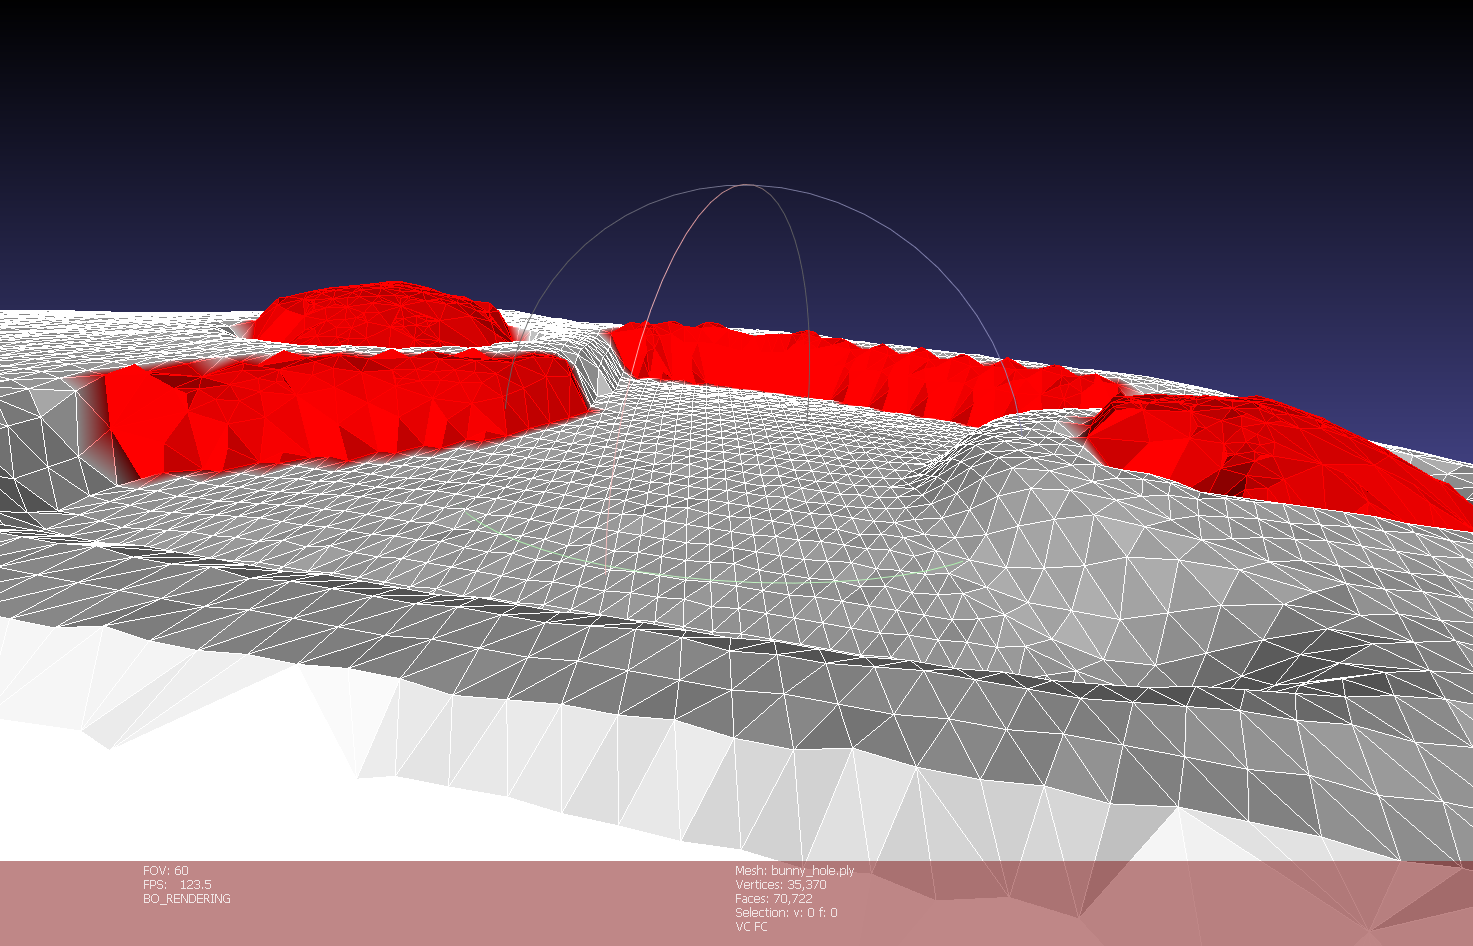
\includegraphics[width=0.55\textwidth]{figures/fig_failure_overshoot.png}
    \caption{Overshoot with \texttt{CurvatureStrength = 1.5} on a sharp Bunny hole.}
    \label{fig:failure-overshoot}
\end{figure}

The second is \emph{under-coverage}: on large holes, with the cow as the worst case, the patch sits on the true surface but does not fully span the removed region, and the reverse-direction Hausdorff distance grows accordingly. Adding interior vertices through smaller \texttt{RefinementFactor} and larger \texttt{DiffusionIterations} reduces the error, but only up to a point: the spherical-cap assumption itself becomes inappropriate for elongated or non-convex hole shapes.

\section{Limitations}

A number of cases lie outside the scope of the current implementation.

The hole detection in Stage~1 walks one boundary loop at a time and assumes a clean 2-manifold input. Holes that share vertices, holes nested inside other holes, and non-manifold edges produce undefined behaviour. In practice, running MeshLab's own non-manifold cleanup before NFD is a workable preprocessing step.

The patch carries vertex colour, averaged from the boundary, but not texture coordinates or material indices. The original Verdera et~al.\ paper extends normal diffusion to texture inpainting, which the present implementation does not.

Sharp features that pass through the hole are not preserved; the patch is uniformly smooth. Recovering them would require detecting crease edges near the boundary and adding them as additional Dirichlet constraints in the diffusion solver, which is more involved than the rest of the pipeline.

The number of diffusion iterations is fixed rather than tolerance-driven. On the test meshes 50 iterations is sufficient, but a residual-based stopping criterion $\|\mathbf{n}^{t+1} - \mathbf{n}^{t}\| < \tau$ would behave more reliably across a wider range of mesh sizes.
